% Study design and analysis workflow. Included from sections/methods.tex (Study design).
% Source: figures/figure1/study_overview_fig.tex (build commands in its header).
\begin{figure}[!t]
\centering
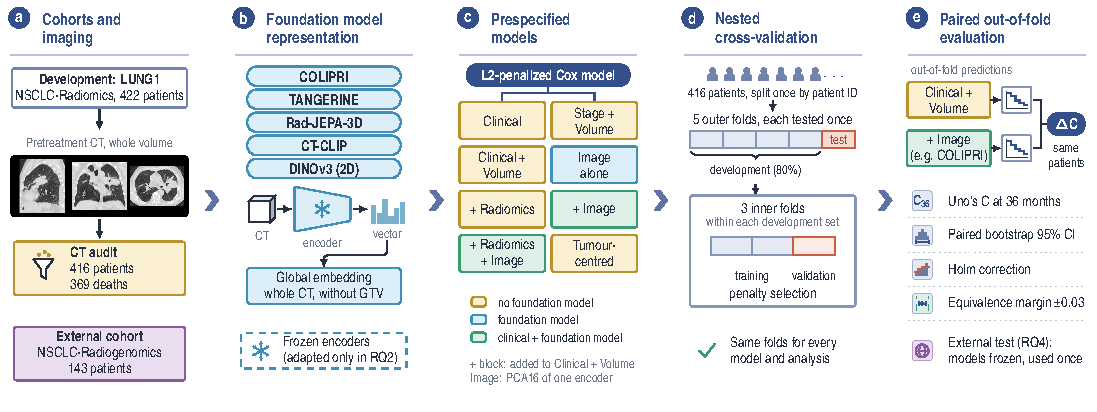
\includegraphics[width=\linewidth]{figures/study_overview.pdf}
\caption{Study design and analysis workflow. (a) LUNG1 provided all development data: after the CT audit, 416 patients had a pretreatment CT, a primary-tumour segmentation (GTV) and overall survival. NSCLC-Radiogenomics was used only for external evaluation. (b) Five foundation models encoded the whole CT with their published preprocessing and without the GTV into one global embedding per patient; the encoders were frozen except in the RQ2 adaptation analyses. (c) The prespecified models: nested clinical models, each adding one block to \model{Clinical+Volume}, the parsimonious \model{Stage+Volume} comparator, each image representation alone and the tumour-centred comparators. In the frozen benchmark, each embedding was reduced to its first 16 principal components (PCA16; 32, PCA32, in a sensitivity analysis), which entered an L2-penalized Cox model. (d) Five outer folds, fixed by patient before any model was fitted, and three inner folds for penalty selection were shared by every model and analysis. (e) Models were compared in pairs on the same test patients, for example \model{Clinical+Volume} with and without COLIPRI, by Uno's C at 36 months with paired bootstrap intervals, Holm correction and equivalence testing. For RQ4, models refitted on all 416 LUNG1 patients were frozen and applied once to the external cohort (purple).}
\label{fig:overview}
\end{figure}
